\chapter{Operational Amplifier}

\section{Operational Amplifier}


\begin{figure}[H]
  \centering
  \begin{subfigure}{.5\textwidth}
    \centering
    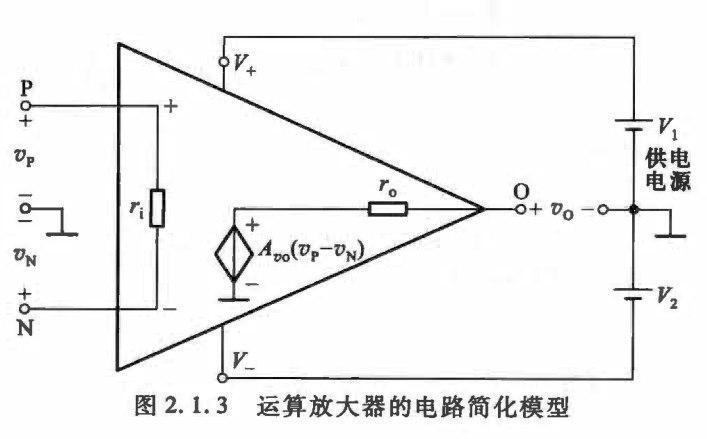
\includegraphics[width=\linewidth]{figures/comparator}
    \caption{the model of an operational amplifier}
    \label{fig:}
  \end{subfigure}%
  \begin{subfigure}{.5\textwidth}
    \centering
    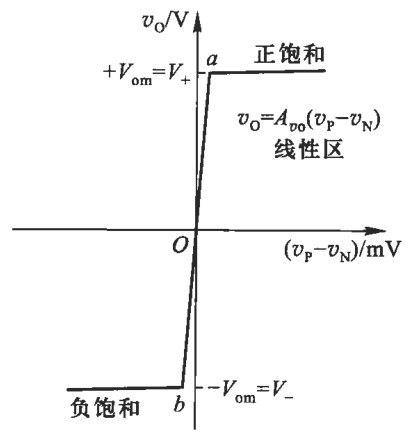
\includegraphics[width=0.6\linewidth]{figures/comparator-voltage-change}
    \caption{How the output voltage varies}
    \label{fig:}
  \end{subfigure}
  \caption{}
  \label{fig:}
\end{figure}

We define $r_i$ as the input impedance, $r_o$ as the output impedance. $v_p$ as the non-inverting input, $v_n$  the inverting input.

Usually, we have $v_p \approx v_n$, $r_i \approx \infty$, $r_o \approx 0$.

Note that the output voltage of a operational amplifier has limits, called \textbf{Bandwidth}. When the input voltage exceeds the limits, it outputs the maximum or minimum value.

\section{Ideal Operational Amplifier}

For ideal operational amplifier:

\begin{itemize}
\item $v_p = v_n$, $i_i = 0$, $r_i = \infty$
\item $r_o = 0$, $v_o = A_{vo} \left( v_p - v_n \right)$
\item $bandwidth = \infty$
  
\end{itemize}

Here is a model which shows all the feature of an ideal operational comparator:

\begin{figure}[H]
  \centering
  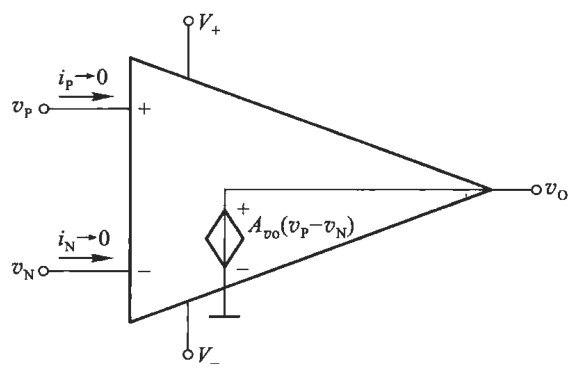
\includegraphics[width=0.5\linewidth]{figures/ideal-comparator}
  \caption{An ideal operational amplifier}
  \label{fig:}
\end{figure}

\section{Closed-looped Amplifier}


Usually operational amplifiers are used with vegetative feedback to ensure its stability. We apply a portion of output voltage to input, reducing the gain of a circuit.

\subsection{Non-inverting Operational Amplifier}

If we connect the inverting input, to the ground, and use the non-inverting input, we get an non-inverting operational amplifier.

The gain of the amplifier is:

\begin{equation*}
  \begin{aligned}
    A_{vo} = \dfrac{R_2 + R_1}{R_1} 
  \end{aligned}
\end{equation*}

The picture below is a non-inverting amplifier.

\begin{figure}[H]
  \centering
  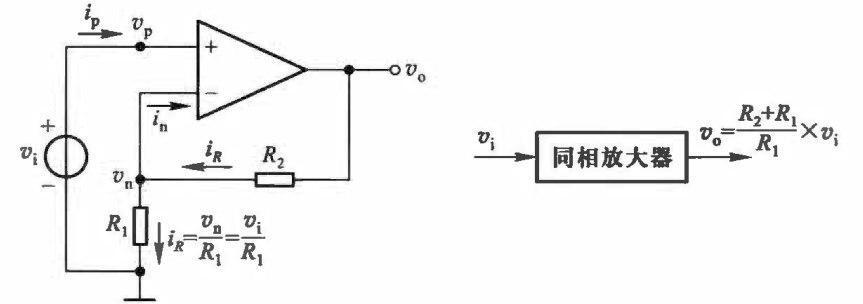
\includegraphics[width=0.9\linewidth]{figures/non-inverting-amplifier}
  \caption{An non-inverting amplifier}
  \label{fig:}
\end{figure}

\begin{equation*}
  \left\{
  \begin{aligned}
    & i_R = \dfrac{v_o - v_n}{R_2} = \dfrac{v_n}{R_1} \\
    & v_n = v_p = v_i
  \end{aligned}
  \right.
\end{equation*}

\begin{equation*}
  \begin{aligned}
    \dfrac{v_o - v_n}{R_2} = \dfrac{v_i}{R_1}  
  \end{aligned}
\end{equation*}

\begin{equation*}
  \begin{aligned}
    A_v = \dfrac{v_o}{v_i} = \dfrac{R_1 + R_2}{R_1}  
  \end{aligned}
\end{equation*}

Note that when $R_2\ll R_1$, $A_{vo} = 1$, $v_i = v_o$.

\subsection{Inverting Operational Amplifier}

If we connect the non-inverting input, to the ground, and use the inverting input, we get an inverting operational amplifier.

The gain of this type of amplifier is:

\begin{equation*}
  \begin{aligned}
    A_{vo} = - \dfrac{R_2}{R_1} 
  \end{aligned}
\end{equation*}

The picture below shows as inverting operational amplifier:

\begin{figure}[H]
  \centering
  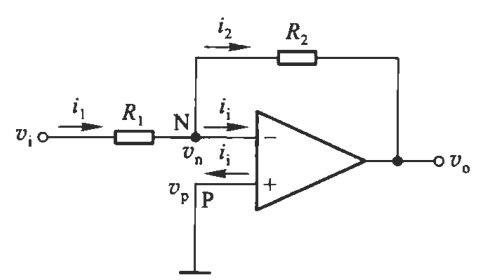
\includegraphics[width=0.4\linewidth]{figures/inverting-amplifier}
  \caption{An inverting amplifier}
  \label{fig:}
\end{figure}

\begin{equation*}
  \left\{
  \begin{aligned}
    & \dfrac{v_o - v_n}{R_2} = \dfrac{v_n - v_i}{R_1} \\
    & v_n = v_p = 0
  \end{aligned}
  \right.
\end{equation*}

\begin{equation*}
  \begin{aligned}
    \dfrac{v_o}{R_2} = \dfrac{- v_i}{R_1}  
  \end{aligned}
\end{equation*}



\begin{equation*}
  \begin{aligned}
    A_v = \dfrac{v_o}{v_i} = - \dfrac{R_2}{R_1}  
  \end{aligned}
\end{equation*}

\section{Applications of operational amplifiers}

\subsection{Subtraction Circuit}

An subtraction circuit can calculate the difference of inverting input and non-inverting input.

\begin{figure}[H]
  \centering
  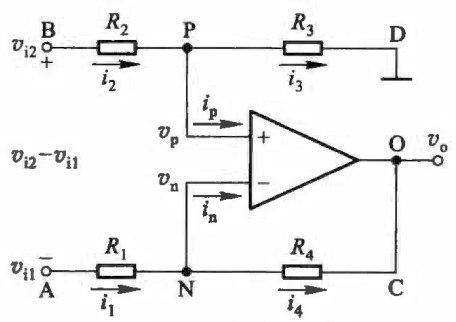
\includegraphics[width=0.4\linewidth]{figures/subtraction-amplifier}
  \caption{A subtraction circuit}
  \label{fig:}
\end{figure}

\begin{equation*}
  \left\{
    \begin{aligned}
      & \dfrac{v_{i2} - v_p}{R_2} = \dfrac{v_p}{R_3} \\
      & \dfrac{v_{i1} - v_n}{R_1} = \dfrac{v_n - v_o}{R_4}  
    \end{aligned}
  \right.
\end{equation*}

\begin{equation*}
  \left\{
  \begin{aligned}
    & R_3 \left( v_{i2} - v_p \right) = R_2 v_p && \Rightarrow v_p = \dfrac{R_3}{R_2 + R_3} v_{i2} \\
    & R_4 \left( v_{i1} - v_n \right) = R_1 \left( v_n - v_0 \right) && \Rightarrow v_n = \dfrac{R_4 v_{i1} + R_1 v_o}{R_4 + R_1}
  \end{aligned}
  \right.
\end{equation*}

\begin{equation*}
  \begin{aligned}
    \dfrac{R_3}{R_2 + R_3} v_{i2} = \dfrac{R_4 v_{i1} + R_1 v_o}{R_4 + R_1}
  \end{aligned}
\end{equation*}

\begin{equation*}
  \begin{aligned}
    \dfrac{R_3 \left( R_4 + R_1 \right)}{R_2 + R_3} v_{i2} = R_4 v_{i1} + R_1 v_o
  \end{aligned}
\end{equation*}

$\Rightarrow$

\begin{equation*}
  \begin{aligned}
    v_o = \dfrac{\dfrac{R_4}{R_1} + 1 }{\dfrac{R_2}{R_3} + 1 } v_{i2} - \dfrac{R_4}{R_1} v_{i1}  = \left( 1 + \dfrac{R_4}{R_1}  \right) \dfrac{\dfrac{R_3}{R_2} }{1 + \dfrac{R_3}{R_2} } v_{i2} - \dfrac{R_4}{R_1} v_{i1} 
  \end{aligned}
\end{equation*}

If $R_4 / R_1 = R_3 / R_2 = r$, then

\begin{equation*}
  \begin{aligned}
    v_o = \left( 1 + r \right) \dfrac{r}{1 + r} v_{i2} - r v_{i1} = r \left( v_{i2} - v_{i1} \right) 
  \end{aligned}
\end{equation*}

\begin{equation*}
  \begin{aligned}
    A_v = r = \dfrac{R_4}{R_1} = \dfrac{R_3}{R_2}  
  \end{aligned}
\end{equation*}

\subsection{Sum Circuit}

An sum circuit adds the inverting input and the non-inverting input.

\begin{figure}[H]
  \centering
  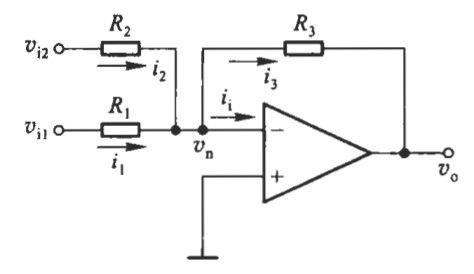
\includegraphics[width=0.4\linewidth]{figures/sum-amplifier}
  \caption{Sum Circuit}
  \label{fig:}
\end{figure}

Similarly, we have

\begin{equation*}
  \left\{
  \begin{aligned}
    & \dfrac{v_{i1} - v_n}{R_1} + \dfrac{v_{i2}- v_n}{R_2} = \dfrac{v_n - v_o}{R_3} \\
    & v_n= v_p = 0
  \end{aligned}
  \right.
\end{equation*}

$\Rightarrow$

\begin{equation*}
  \begin{aligned}
    \dfrac{v_{i1}}{R_1} + \dfrac{v_{i2}}{R_2} = \dfrac{- v_o}{R_3} \\
  \end{aligned}
\end{equation*}

\begin{equation*}
  \begin{aligned}
    v_o = - \left( \dfrac{R_3}{R_1} v_{i1} + \dfrac{R_3}{R_2} v_{i2} \right) 
  \end{aligned}
\end{equation*}

When we set

\begin{equation*}
  \begin{aligned}
    R_1 = R_2 = R_3
  \end{aligned}
\end{equation*}

We have

\begin{equation*}
  \begin{aligned}
    v_o = - \left( v_{i1} + v_{i2} \right)
  \end{aligned}
\end{equation*}

\subsection{Integrating Circuit}

\begin{figure}[H]
  \centering
  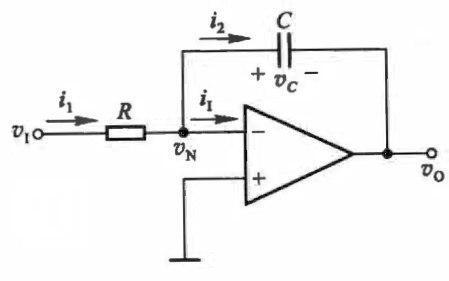
\includegraphics[width=0.4\linewidth]{figures/integrating-circuit}
  \caption{integrating circuit}
  \label{fig:}
\end{figure}

\begin{equation*}
  \begin{aligned}
    C = \dfrac{Q}{U} \Rightarrow U = \dfrac{Q}{C} = \dfrac{1}{C} \int I \md t = \dfrac{1}{C} \int \dfrac{v_i}{R} \md t = \dfrac{1}{RC} \int v_i \md t
  \end{aligned}
\end{equation*}

\begin{equation*}
  \begin{aligned}
    0 - v_o = U
  \end{aligned}
\end{equation*}

$\Rightarrow$

\begin{equation*}
  \begin{aligned}
    v_o = - \dfrac{1}{RC} \int v_i \md t
  \end{aligned}
\end{equation*}

We define

\begin{equation*}
  \begin{aligned}
    \tau = RC
  \end{aligned}
\end{equation*}

Then

\begin{equation*}
  \begin{aligned}
    - v_o = \dfrac{1}{\tau} \int v_{1} \mathrm{d} t
  \end{aligned}
\end{equation*}

\subsection{Differential Circuit}

\begin{figure}[H]
  \centering
  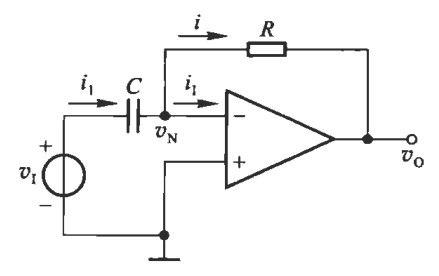
\includegraphics[width=0.4\linewidth]{figures/differential-circuit}
  \caption{differential circuit}
  \label{fig:}
\end{figure}

\begin{equation*}
  \left\{
  \begin{aligned}
    i_i &= \dfrac{\md Q}{\md t} = C \dfrac{\md v_i}{\md t}  \\
    i &= \dfrac{v_o}{R} \\
    i_i &= i
  \end{aligned}
  \right.
\end{equation*}

$\Rightarrow$

\begin{equation*}
  \begin{aligned}
    - v_o = R C \dfrac{\mathrm{d} v_i}{\mathrm{d} t} = \tau \dfrac{\md v_i}{\md t} 
  \end{aligned}
\end{equation*}


%%% Local Variables:
%%% mode: latex
%%% TeX-master: "main"
%%% End:
